\documentclass[10pt]{beamer}

\usetheme{CambridgeUS}
\usepackage[english, russian]{babel}
\usepackage[utf8]{inputenc}
\usepackage{caption}
\usepackage{etoolbox}
\usepackage{multicol}
\usepackage{listings}
\usepackage{color}

\definecolor{mygreen}{rgb}{0,0.6,0}
\lstset{
  basicstyle=\ttfamily\footnotesize,        % the size of the fonts that are used for the code
  breaklines=true,                 % automatic line breaking only at whitespace
  captionpos=b,                    % sets the caption-position to bottom
  commentstyle=\color{mygreen},    % comment style
  keywordstyle=\color{blue},       % keyword style
  stringstyle=\color{red},     % string literal style
  showstringspaces=false,
  morekeywords={include, printf},
  texcl=true     %<---- added
}


\title[\href{https://goo.gl/NRgp8K}{https://goo.gl/NRgp8K} (Term 3)]{Руководство по Git}
\author[Гусев Илья]{Гусев Илья}
\institute[МФТИ] 
{Московский физико-технический институт\\*}
\date{Москва, 2017}
\subject{Computer Science}

\begin{document}

\begin{frame}
  \titlepage
\end{frame}

\begin{frame}{Содержание}
\tableofcontents
\end{frame}

\section{Введение}

\subsection{VCS}
\begin{frame}[fragile]{VCS}{Что такое VCS (система контроля версий)?}
\begin{multicols}{2}
Простой сценарий:
\begin{enumerate}
\item Создание файла
\item Изменение файла
\item Сохранение файла
\item Goto 2
\end{enumerate}
\vfill\eject
Обычный сценарий:
\begin{enumerate}
\item Создание файла
\item Изменение файла
\item Сохранение файла
\item Изменение файла
\item Сохранение файла
\item Захотелось вернуться в состояние 3
\end{enumerate}
Решается резервным копированием.
\end{multicols}
\end{frame}

\begin{frame}[fragile]{VCS}{Что такое VCS (система контроля версий)?}
\begin{multicols}{2}
Сложный сценарий - 2 человека работают над одним файлом:
\begin{enumerate}
\item Создание файла (1 человек)
\item Изменение файла (1 человек)
\item Сохранение файла (1 человек)
\item Получение файла (2 человек)
\item Изменение файла (1 человек)
\item Изменение файла (2 человек)
\item Сохранение файла (2 человек)
\item Получение файла (1 человек), слияние изменений
\item Сохранение файла (1 человек)
\item Получение файла (2 человек)
\end{enumerate}
\end{multicols}
А ещё может понадобиться возвращение в 3, 7, 9...
\end{frame}

\begin{frame}[fragile]{VCS}{Что такое VCS (система контроля версий)?}
Система контроля версий - софт, который позволяет работать в рамках таких сложных сценариев, когда десятки людей вносят изменения в одни и те же файлы. В сочетании с CI (Continuous Integration, непрерывная интеграция) - основа инфраструктуры при разработке почти любого программного продукта. 

Можно использовать не только над исходным кодом, а в принципе над любыми текстовыми файлами (и не только текстовыми).
\end{frame}

\subsection{Варинты VCS}
\begin{frame}[fragile]{Варинты VCS}{Subversion (SVN) vs Git}
\begin{enumerate}
\item \textbf{Централизованная  vs распределённая.} У SVN одно хранилище, там лежит полная история, на локальных машинах - последняя версия (working copy). В случае Git'а - каждая машина имеет полную копию репозитория со всей историей. Сервер - такая же машина, только лишь с возможностью pull, push и ограничениями доступа.
\item \textbf{Git - ветки}. У Git'а намного более удобная система ветвления. Есть возможность создавать ветки локально (для отдельных фич, например), и потом их целиком сливать на сервер. Ветки очень лёгкие, по сути - всего лишь указатель на коммит.
\item  Первый выпуск: 2000 vs 2005.
\end{enumerate}
\end{frame}

\section{Git}
\subsection{Установка}

\begin{frame}[fragile]{Git}{Установка}
\begin{enumerate}
\item Скачивание: \href{https://git-scm.com/downloads}{\texttt{https://git-scm.com/downloads}}
\item Установка...
\item Первоначальная настройка: \\
\texttt{git config --global user.name <ваше имя>}\\
\texttt{git config --global user.email <ваша почта>}\\
\texttt{git config --global core.editor <ваш любимый редактор>}\\
\texttt{git config --list}
\end{enumerate}
\end{frame}

\subsection{Создание или клонирование репозитория}
\begin{frame}[fragile]{Git}{Создание или клонирование репозитория}
\begin{enumerate}
\item Создание репозитория:\\
\texttt{cd <нужная папка>}\\
\texttt{git init}\\

\item Клонирование репозитория: \\
\texttt{cd <папка, уровнем выше нужной>}\\
\texttt{git clone <адрес репозитория> <имя нужной папки>}\\
\end{enumerate}
\end{frame}

\subsection{Отслеживание файлов}
\begin{frame}[fragile]{Git}{Отслеживание файлов}
\begin{enumerate}
\item Добавление файла в индекс:\\
\texttt{git add <имя файла> }\\
\item Добавление всех файлов в индекс:\\
\texttt{git add -a }\\
\item Удаление файла из индекса:\\
\texttt{git rm <имя файла> }\\
\item Фиксация изменений\\
\texttt{git commit -m "Сообщение при коммите" }\\
\item Добавление всех файлов + фиксация\\
\texttt{git commit -a -m "Сообщение при коммите" }\\
\end{enumerate}
\end{frame}

\begin{frame}[fragile]{Git}{.gitignore}
Файл в корне репозитория, определяет, какие файлы автоматически игнорируются.
Пример из git-book:
\begin{lstlisting}[language=bash]
# комментарий — эта строка игнорируется
# не обрабатывать файлы, имя которых заканчивается на .a
*.a
# НО отслеживать файл lib.a, несмотря на то, что мы игнорируем все .a файлы с помощью предыдущего правила
!lib.a
# игнорировать только файл TODO находящийся в корневом каталоге, не относится к файлам вида subdir/TODO
/TODO
# игнорировать все файлы в каталоге build/
build/
# игнорировать doc/notes.txt, но не doc/server/arch.txt
doc/*.txt
# игнорировать все .txt файлы в каталоге doc/
doc/**/*.txt
\end{lstlisting}
\end{frame}

\subsection{Отмена изменений}
\begin{frame}[fragile]{Git}{Отмена изменений}
\begin{enumerate}
\item Исправление последнего коммита:\\
\texttt{git commit --amend}\\
Пример:\\
\texttt{git commit -m "Сообщение при коммите"}\\
\texttt{git add <забытый файл>}\\
\texttt{git commit ---amend}\\

\item Отмена индексации (soft reset) до последнего коммита:\\
\texttt{git reset ---soft HEAD}\\

\item Отмена всех изменений (hard reset) до последнего коммита:\\
\texttt{git reset ---hard HEAD}\\

\item Отмена всех изменений в файле до последнего коммита:\\
\texttt{git checkout --- <имя файла> }\\

\item Отмена всех изменений (hard reset) до N-ого коммита с конца:\\
\texttt{git reset ---hard HEAD$\sim$N}\\
\end{enumerate}
\end{frame}


\subsection{Служебные команды}
\begin{frame}[fragile]{Git}{Служебные команды}
\begin{enumerate}
\item Лог коммитов:\\
\texttt{git log}\\

\item Лог коммитов (красивый, с веточками):\\
\texttt{git log ---graph}\\

\item Статус индекса:\\
\texttt{git status}\\

\item Просмотр изменений:\\
\texttt{git diff}\\

\item Просмотр индексирвоанных изменений:\\
\texttt{git diff ---cached}\\

\item Сжатие (происходит автоматически при push):\\
\texttt{git gc}\\

\end{enumerate}
\end{frame}


\subsection{Удалённые репозитории}
\begin{frame}[fragile]{Git}{Удалённые репозитории}
\begin{enumerate}
\item Добавление удалённого репозитория:\\
\texttt{git remote add <сокращение> <url>}\\

\item Получение новых изменений:\\
\texttt{git fetch}\\

\item Получение новых изменений (с автослиянием):\\
\texttt{git pull}\\

\item Получение новых изменений из конкретной ветки (с автослиянием)\\
\texttt{git pull <имя репозитория> <имя ветки>}\\

\item Отправка изменений:\\
\texttt{git push <имя репозитория> <имя ветки>}\\
\end{enumerate}
\end{frame}


\subsection{Ветки}
\begin{frame}[fragile]{Git}{Ветки}
\begin{multicols}{2}
\begin{enumerate}
\item Каждый коммит характеризуется несколькими основными вещами: хеш (на картинке - его первые 5 цифр), автор, дата.
\item HEAD -  метка показывающая на текущий коммит, который мы сейчас изменяем.
\item Ветка - формально, указатель на коммит. Иногда ещё подразумевают всю историю до этого коммита.
\end{enumerate}
\vfill\eject
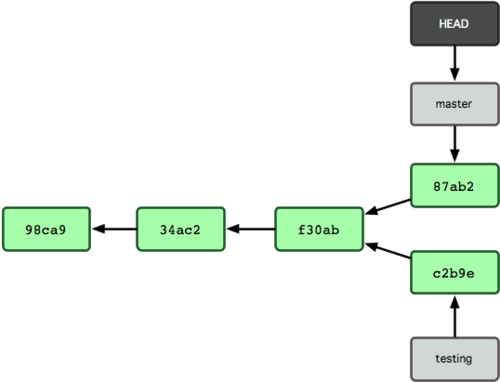
\includegraphics[width=5cm, height=4cm]{Term_3/Source/Pictures/branches.png}
\end{multicols}
\end{frame}

\begin{frame}[fragile]{Git}{Операции с ветками}
\begin{enumerate}
\item Создание ветки (указывает на текущий коммит):\\
\texttt{git branch <название ветки>}\\
\item Переход на ветку:\\
\texttt{git checkout <название ветки>}\\
\item Слияние:\\
\texttt{git merge <из какой ветки>}\\
\item При успешном разрешении конфликтов слияния:\\
\texttt{git commit -a}\\
\end{enumerate}
\end{frame}

\section{Workflow}
\subsection{Репозиторий}
\begin{frame}[fragile]{Workflow}{Репозиторий}
\begin{enumerate}
\item Сервер - Bitbucket.
\item Создаёте приватный репозиторий.
\item Добавляете семинаристов (Settings -> User and group access).
\item Даёте админские права.
\item Вся работа в рамках этого репозитория.
\item Без пройденного ревью на Bitbucket задача не засчитывается!
\item Не забудьте про .gitignore!
\end{enumerate}
\end{frame}

\subsection{Ветки}
\begin{frame}[fragile]{Workflow}{Устройство веток в вашем репозитории}
\begin{enumerate}
\item master - ветка, куда вливается подтверждённый семинаристом код.
\item Для каждой задачи отдельная ветка. Стандартный сценарий при настроенном репозитории:\\
\begin{enumerate}
    \item \texttt{git checkout master}\\
    \item \texttt{git checkout -b <название или номер задачи>}\\
    \item \texttt{делаете изменения, сдаёте в контесте}\\
    \item \texttt{git commit -a -m <сообщение>}\\
    \item \texttt{git push <имя репозитория> <имя ветки>}\\
\end{enumerate}
\end{enumerate}
\end{frame}

\begin{frame}[fragile]{Workflow}{Устройство веток в вашем репозитории}
\begin{enumerate}
\item Когда всё готово, делаете pull request в master. Названия pull request'ов должны быть по шаблону:\\
\texttt{[Имя Фамилия] ДЗ-<номер ДЗ>, <название задачи>.} 
\item В описании pull request'а должна быть ссылка на успешную посылку в контесте.
\item Семинаристы делают ревью, вы исправляете замечания.

\end{enumerate}
\end{frame}

\appendix
\section<presentation>*{\appendixname}
\subsection<presentation>*{Useful links}

\begin{frame}[allowframebreaks]
  \frametitle<presentation>{Полезные ссылки}
    
  \begin{thebibliography}{10}
{
  \beamertemplatebookbibitems
  % Start with overview books.


  \bibitem{Pro Git}
  \texttt{Pro Git}
  \newblock \href{https://git-scm.com/book/ru/v1}{\texttt{https://git-scm.com/book/ru/v1}}
}
    
  \end{thebibliography}
\end{frame}

\end{document}


